% !TeX program = pdflatex
% Self-contained editable source. All examples use the existing local collection.
\documentclass[a4paper]{article}
\usepackage[margin=0pt]{geometry}
\usepackage[T1]{fontenc}
\usepackage{lmodern}
\makeatletter\input{t1lmss.fd}\makeatother
\DeclareFontShape{T1}{lmss}{m}{n}{<-> ec-lmss9}{}
\usepackage{tikz}
\usepackage{xcolor}
\usepackage[hidelinks]{hyperref}
\renewcommand{\familydefault}{\sfdefault}
\pagestyle{empty}
\setlength{\parindent}{0pt}
\setlength{\topskip}{0pt}
\date{}
\hypersetup{pdftitle={KOS Computing Structures},pdfsubject={Local evidence tables and organizational structures}}
\definecolor{KInk}{HTML}{182D43}
\definecolor{KMuted}{HTML}{526375}
\definecolor{KLine}{HTML}{CCD6DE}
\definecolor{KTable}{HTML}{EEF2F6}
\definecolor{KBlue}{HTML}{28679E}
\definecolor{KTeal}{HTML}{147A7A}
\definecolor{KOrange}{HTML}{A76329}
\definecolor{KViolet}{HTML}{715B99}
\begin{document}
\begin{tikzpicture}[remember picture,overlay,x=1bp,y=-1bp]\begin{scope}[shift={(current page.north west)}]
\node[anchor=north west,inner sep=0pt,text width=523.28bp,align=center,text=KInk,font=\fontsize{19}{22}\selectfont\sffamily] at (36,27){\bfseries KOS Computing Structures};
\node[anchor=north west,inner sep=0pt,text width=523.28bp,align=center,text=KMuted,font=\fontsize{9.5}{12}\selectfont\sffamily] at (36,53){One computing theme, with local context. Tables precede their corresponding diagrams.};
\draw[draw=KLine,line width=0.6bp] (36,77) -- (559.28,77);
\node[anchor=north west,inner sep=0pt,text width=523.28bp,align=center,text=KMuted,font=\fontsize{8}{10}\selectfont\sffamily] at (36,820){1 / 5};
\node[anchor=north west,inner sep=0pt,text width=28bp,align=left,text=KOrange,font=\fontsize{10}{13}\selectfont\sffamily] at (36,94){\bfseries 01};
\node[anchor=north west,inner sep=0pt,text width=493bp,align=left,text=KInk,font=\fontsize{13.3}{16}\selectfont\sffamily] at (66,94){\bfseries DDC: observed labels and document descriptions};
\node[anchor=north west,inner sep=0pt,text width=523bp,align=left,text=KMuted,font=\fontsize{8.6}{10.8}\selectfont\sffamily] at (36,116){Labels are corpus assignments. Descriptions below are document-text excerpts, not official class definitions.};
\path[fill=KTable] (36,143) rectangle (559,164);
\node[anchor=north west,inner sep=0pt,text width=33bp,align=left,text=KInk,font=\fontsize{8.5}{10}\selectfont\sffamily] at (41,148){\bfseries Label};
\node[anchor=north west,inner sep=0pt,text width=122bp,align=left,text=KInk,font=\fontsize{8.5}{10}\selectfont\sffamily] at (84,148){\bfseries Document title};
\node[anchor=north west,inner sep=0pt,text width=278bp,align=left,text=KInk,font=\fontsize{8.5}{10}\selectfont\sffamily] at (216,148){\bfseries Description (excerpt)};
\node[anchor=north west,inner sep=0pt,text width=50bp,align=left,text=KInk,font=\fontsize{8.5}{10}\selectfont\sffamily] at (504,148){\bfseries D / A row};
\draw[draw=KLine,line width=0.6bp] (36,164) -- (559,164);
\node[anchor=north west,inner sep=0pt,text width=33bp,align=left,text=KInk,font=\fontsize{8.4}{10.7}\selectfont\sffamily] at (41,169){004};
\node[anchor=north west,inner sep=0pt,text width=122bp,align=left,text=KInk,font=\fontsize{8.4}{10.7}\selectfont\sffamily] at (84,169){Computer programming};
\node[anchor=north west,inner sep=0pt,text width=278bp,align=left,text=KInk,font=\fontsize{8.4}{10.7}\selectfont\sffamily] at (216,169){There are some unobvious dead lock problems caused by inappropriate acquiring and releasing resources among current transactions. At first, this...};
\node[anchor=north west,inner sep=0pt,text width=50bp,align=left,text=KInk,font=\fontsize{8.4}{10.7}\selectfont\sffamily] at (504,169){5384};
\draw[draw=KLine,line width=0.6bp] (36,212) -- (559,212);
\node[anchor=north west,inner sep=0pt,text width=33bp,align=left,text=KInk,font=\fontsize{8.4}{10.7}\selectfont\sffamily] at (41,217){005};
\node[anchor=north west,inner sep=0pt,text width=122bp,align=left,text=KInk,font=\fontsize{8.4}{10.7}\selectfont\sffamily] at (84,217){Python pocket reference};
\node[anchor=north west,inner sep=0pt,text width=278bp,align=left,text=KInk,font=\fontsize{8.4}{10.7}\selectfont\sffamily] at (216,217){Updated for both Python 3.4 and 2.7, this guide provides concise information on Python types and statements, special method names, built-in...};
\node[anchor=north west,inner sep=0pt,text width=50bp,align=left,text=KInk,font=\fontsize{8.4}{10.7}\selectfont\sffamily] at (504,217){6303};
\draw[draw=KLine,line width=0.6bp] (36,260) -- (559,260);
\node[anchor=north west,inner sep=0pt,text width=33bp,align=left,text=KInk,font=\fontsize{8.4}{10.7}\selectfont\sffamily] at (41,265){006};
\node[anchor=north west,inner sep=0pt,text width=122bp,align=left,text=KInk,font=\fontsize{8.4}{10.7}\selectfont\sffamily] at (84,265){Machine learning with SPARK and Python};
\node[anchor=north west,inner sep=0pt,text width=278bp,align=left,text=KInk,font=\fontsize{8.4}{10.7}\selectfont\sffamily] at (216,265){Machine Learning with Spark and Python Essential Techniques for Predictive Analytics, Second Edition simplifies ML for practical uses by...};
\node[anchor=north west,inner sep=0pt,text width=50bp,align=left,text=KInk,font=\fontsize{8.4}{10.7}\selectfont\sffamily] at (504,265){6873};
\draw[draw=KLine,line width=0.6bp] (36,308) -- (559,308);
\node[anchor=center,draw=KOrange,fill=KOrange!5,rounded corners=3bp,line width=.7bp,align=center,inner sep=4bp,text width=144bp,minimum height=36bp,text=KInk,font=\fontsize{9}{10.7}\selectfont\sffamily] (ddoc0) at (117,333){{\bfseries Computer programming}};
\node[anchor=center,draw=KOrange,fill=KOrange!5,rounded corners=3bp,line width=.7bp,align=center,inner sep=4bp,text width=66bp,minimum height=26bp,text=KInk,font=\fontsize{9}{10.7}\selectfont\sffamily] (dcode0) at (117,389){{\bfseries 004}};
\draw[->,>=stealth,draw=KOrange,line width=.9bp] (ddoc0.south) -- node[pos=0.5,fill=white,inner sep=2bp,text=KOrange,font=\fontsize{7.8}{9}\selectfont\sffamily] {assignment} (dcode0.north);
\node[anchor=center,draw=KOrange,fill=KOrange!13,rounded corners=3bp,line width=.7bp,align=center,inner sep=4bp,text width=144bp,minimum height=36bp,text=KInk,font=\fontsize{9}{10.7}\selectfont\sffamily] (ddoc1) at (298,333){{\bfseries Python pocket reference}};
\node[anchor=center,draw=KOrange,fill=KOrange!13,rounded corners=3bp,line width=.7bp,align=center,inner sep=4bp,text width=66bp,minimum height=26bp,text=KInk,font=\fontsize{9}{10.7}\selectfont\sffamily] (dcode1) at (298,389){{\bfseries 005}};
\draw[->,>=stealth,draw=KOrange,line width=.9bp] (ddoc1.south) -- node[pos=0.5,fill=white,inner sep=2bp,text=KOrange,font=\fontsize{7.8}{9}\selectfont\sffamily] {assignment} (dcode1.north);
\node[anchor=center,draw=KOrange,fill=KOrange!5,rounded corners=3bp,line width=.7bp,align=center,inner sep=4bp,text width=144bp,minimum height=36bp,text=KInk,font=\fontsize{9}{10.7}\selectfont\sffamily] (ddoc2) at (479,333){{\bfseries Machine learning with SPARK and Python}};
\node[anchor=center,draw=KOrange,fill=KOrange!5,rounded corners=3bp,line width=.7bp,align=center,inner sep=4bp,text width=66bp,minimum height=26bp,text=KInk,font=\fontsize{9}{10.7}\selectfont\sffamily] (dcode2) at (479,389){{\bfseries 006}};
\draw[->,>=stealth,draw=KOrange,line width=.9bp] (ddoc2.south) -- node[pos=0.5,fill=white,inner sep=2bp,text=KOrange,font=\fontsize{7.8}{9}\selectfont\sffamily] {assignment} (dcode2.north);
\node[anchor=north west,inner sep=0pt,text width=523bp,align=left,text=KMuted,font=\fontsize{8.5}{11}\selectfont\sffamily] at (36,412){004, 005 and 006 are neighboring observed codes only. No common parent or official caption is supplied.};
\node[anchor=north west,inner sep=0pt,text width=523bp,align=left,text=KMuted,font=\fontsize{7.9}{10}\selectfont\sffamily] at (36,436){D / A: DDC\_Prepared\_Documents\_001.xlsx / DDC\_Prepared\_Assignments\_001.xlsx, Documents / Assignments; rows above. Labels: DDC\_Prepared.xlsx, Units 6-8.};
\node[anchor=north west,inner sep=0pt,text width=28bp,align=left,text=KTeal,font=\fontsize{10}{13}\selectfont\sffamily] at (36,467){\bfseries 02};
\node[anchor=north west,inner sep=0pt,text width=493bp,align=left,text=KInk,font=\fontsize{13.3}{16}\selectfont\sffamily] at (66,467){\bfseries UDC: neighboring concepts with a shared broader concept};
\path[fill=KTable] (36,491) rectangle (559,512);
\node[anchor=north west,inner sep=0pt,text width=51bp,align=left,text=KInk,font=\fontsize{8.5}{10}\selectfont\sffamily] at (41,496){\bfseries Notation};
\node[anchor=north west,inner sep=0pt,text width=257bp,align=left,text=KInk,font=\fontsize{8.5}{10}\selectfont\sffamily] at (102,496){\bfseries Preferred label};
\node[anchor=north west,inner sep=0pt,text width=59bp,align=left,text=KInk,font=\fontsize{8.5}{10}\selectfont\sffamily] at (369,496){\bfseries Broader};
\node[anchor=north west,inner sep=0pt,text width=116bp,align=left,text=KInk,font=\fontsize{8.5}{10}\selectfont\sffamily] at (438,496){\bfseries Source rows};
\draw[draw=KLine,line width=0.6bp] (36,512) -- (559,512);
\node[anchor=north west,inner sep=0pt,text width=51bp,align=left,text=KInk,font=\fontsize{8.4}{10.7}\selectfont\sffamily] at (41,517){004};
\node[anchor=north west,inner sep=0pt,text width=257bp,align=left,text=KInk,font=\fontsize{8.4}{10.7}\selectfont\sffamily] at (102,517){Computer science and technology. Computing. Data processing};
\node[anchor=north west,inner sep=0pt,text width=59bp,align=left,text=KInk,font=\fontsize{8.4}{10.7}\selectfont\sffamily] at (369,517){context only};
\node[anchor=north west,inner sep=0pt,text width=116bp,align=left,text=KInk,font=\fontsize{8.4}{10.7}\selectfont\sffamily] at (438,517){U657};
\draw[draw=KLine,line width=0.6bp] (36,542) -- (559,542);
\node[anchor=north west,inner sep=0pt,text width=51bp,align=left,text=KInk,font=\fontsize{8.4}{10.7}\selectfont\sffamily] at (41,547){004.4};
\node[anchor=north west,inner sep=0pt,text width=257bp,align=left,text=KInk,font=\fontsize{8.4}{10.7}\selectfont\sffamily] at (102,547){Software};
\node[anchor=north west,inner sep=0pt,text width=59bp,align=left,text=KInk,font=\fontsize{8.4}{10.7}\selectfont\sffamily] at (369,547){004};
\node[anchor=north west,inner sep=0pt,text width=116bp,align=left,text=KInk,font=\fontsize{8.4}{10.7}\selectfont\sffamily] at (438,547){U678 / S3358};
\draw[draw=KLine,line width=0.6bp] (36,564) -- (559,564);
\node[anchor=north west,inner sep=0pt,text width=51bp,align=left,text=KInk,font=\fontsize{8.4}{10.7}\selectfont\sffamily] at (41,569){004.42};
\node[anchor=north west,inner sep=0pt,text width=257bp,align=left,text=KInk,font=\fontsize{8.4}{10.7}\selectfont\sffamily] at (102,569){Computer programming. Computer programs};
\node[anchor=north west,inner sep=0pt,text width=59bp,align=left,text=KInk,font=\fontsize{8.4}{10.7}\selectfont\sffamily] at (369,569){004.4};
\node[anchor=north west,inner sep=0pt,text width=116bp,align=left,text=KInk,font=\fontsize{8.4}{10.7}\selectfont\sffamily] at (438,569){U683 / S3384};
\draw[draw=KLine,line width=0.6bp] (36,592) -- (559,592);
\node[anchor=north west,inner sep=0pt,text width=51bp,align=left,text=KInk,font=\fontsize{8.4}{10.7}\selectfont\sffamily] at (41,597){004.43};
\node[anchor=north west,inner sep=0pt,text width=257bp,align=left,text=KInk,font=\fontsize{8.4}{10.7}\selectfont\sffamily] at (102,597){Computer languages};
\node[anchor=north west,inner sep=0pt,text width=59bp,align=left,text=KInk,font=\fontsize{8.4}{10.7}\selectfont\sffamily] at (369,597){004.4};
\node[anchor=north west,inner sep=0pt,text width=116bp,align=left,text=KInk,font=\fontsize{8.4}{10.7}\selectfont\sffamily] at (438,597){U684 / S3388};
\draw[draw=KLine,line width=0.6bp] (36,614) -- (559,614);
\node[anchor=north west,inner sep=0pt,text width=51bp,align=left,text=KInk,font=\fontsize{8.4}{10.7}\selectfont\sffamily] at (41,619){004.45};
\node[anchor=north west,inner sep=0pt,text width=257bp,align=left,text=KInk,font=\fontsize{8.4}{10.7}\selectfont\sffamily] at (102,619){System software};
\node[anchor=north west,inner sep=0pt,text width=59bp,align=left,text=KInk,font=\fontsize{8.4}{10.7}\selectfont\sffamily] at (369,619){004.4};
\node[anchor=north west,inner sep=0pt,text width=116bp,align=left,text=KInk,font=\fontsize{8.4}{10.7}\selectfont\sffamily] at (438,619){U685 / S3392};
\draw[draw=KLine,line width=0.6bp] (36,636) -- (559,636);
\node[anchor=center,draw=KTeal,fill=KTeal!5,rounded corners=3bp,line width=.7bp,align=center,inner sep=4bp,text width=144bp,minimum height=36bp,text=KInk,font=\fontsize{9}{10.7}\selectfont\sffamily] (usoftware) at (270,667){{\bfseries 004.4 - Software}};
\node[anchor=center,draw=KTeal,fill=KTeal!5,rounded corners=3bp,line width=.7bp,align=center,inner sep=4bp,text width=132bp,minimum height=36bp,text=KInk,font=\fontsize{9}{10.7}\selectfont\sffamily] (ucomputing) at (486,667){{\bfseries 004 - Computing}\\[-1pt]{\fontsize{7.8}{9.3}\selectfont label shortened in diagram}};
\draw[->,>=stealth,draw=KTeal,line width=.9bp] (usoftware.east) -- node[pos=0.5,fill=white,inner sep=2bp,text=KTeal,font=\fontsize{7.8}{9}\selectfont\sffamily] {broader} (ucomputing.west);
\node[anchor=center,draw=KTeal,fill=KTeal!5,rounded corners=3bp,line width=.7bp,align=center,inner sep=4bp,text width=144bp,minimum height=38bp,text=KInk,font=\fontsize{9}{10.7}\selectfont\sffamily] (uprogram) at (117,750){{\bfseries 004.42}\\[-1pt]{\fontsize{7.8}{9.3}\selectfont Computer programming}};
\draw[->,>=stealth,draw=KTeal,line width=.9bp] (uprogram.north) -- node[pos=0.48,fill=white,inner sep=2bp,text=KTeal,font=\fontsize{7.8}{9}\selectfont\sffamily] {broader} (usoftware.south);
\node[anchor=center,draw=KTeal,fill=KTeal!13,rounded corners=3bp,line width=.7bp,align=center,inner sep=4bp,text width=144bp,minimum height=38bp,text=KInk,font=\fontsize{9}{10.7}\selectfont\sffamily] (ulanguage) at (298,750){{\bfseries 004.43}\\[-1pt]{\fontsize{7.8}{9.3}\selectfont Computer languages}};
\draw[->,>=stealth,draw=KTeal,line width=.9bp] (ulanguage.north) -- node[pos=0.48,fill=white,inner sep=2bp,text=KTeal,font=\fontsize{7.8}{9}\selectfont\sffamily] {broader} (usoftware.south);
\node[anchor=center,draw=KTeal,fill=KTeal!5,rounded corners=3bp,line width=.7bp,align=center,inner sep=4bp,text width=144bp,minimum height=38bp,text=KInk,font=\fontsize{9}{10.7}\selectfont\sffamily] (usystem) at (479,750){{\bfseries 004.45}\\[-1pt]{\fontsize{7.8}{9.3}\selectfont System software}};
\draw[->,>=stealth,draw=KTeal,line width=.9bp] (usystem.north) -- node[pos=0.48,fill=white,inner sep=2bp,text=KTeal,font=\fontsize{7.8}{9}\selectfont\sffamily] {broader} (usoftware.south);
\node[anchor=north west,inner sep=0pt,text width=523bp,align=left,text=KMuted,font=\fontsize{8}{10}\selectfont\sffamily] at (36,780){All arrows: skos:broader, from specific to broader. Source: UDC\_Summary\_Prepared.xlsx; U = Units, S = Statements. The table preserves the full preferred labels.};
\end{scope}\end{tikzpicture}\null\newpage
\begin{tikzpicture}[remember picture,overlay,x=1bp,y=-1bp]\begin{scope}[shift={(current page.north west)}]
\node[anchor=north west,inner sep=0pt,text width=523.28bp,align=center,text=KInk,font=\fontsize{19}{22}\selectfont\sffamily] at (36,27){\bfseries Schedule Context and Subject Headings};
\node[anchor=north west,inner sep=0pt,text width=523.28bp,align=center,text=KMuted,font=\fontsize{9.5}{12}\selectfont\sffamily] at (36,53){A shared level requires a recorded common parent; adjacency alone does not establish hierarchy.};
\draw[draw=KLine,line width=0.6bp] (36,77) -- (559.28,77);
\node[anchor=north west,inner sep=0pt,text width=523.28bp,align=center,text=KMuted,font=\fontsize{8}{10}\selectfont\sffamily] at (36,820){2 / 5};
\node[anchor=north west,inner sep=0pt,text width=28bp,align=left,text=KBlue,font=\fontsize{10}{13}\selectfont\sffamily] at (36,94){\bfseries 03};
\node[anchor=north west,inner sep=0pt,text width=493bp,align=left,text=KInk,font=\fontsize{13.3}{16}\selectfont\sffamily] at (66,94){\bfseries LCC: Python and adjacent entries in the printed schedule};
\path[fill=KTable] (36,122) rectangle (559,143);
\node[anchor=north west,inner sep=0pt,text width=30bp,align=left,text=KInk,font=\fontsize{8.5}{10}\selectfont\sffamily] at (41,127){\bfseries Row};
\node[anchor=north west,inner sep=0pt,text width=99bp,align=left,text=KInk,font=\fontsize{8.5}{10}\selectfont\sffamily] at (81,127){\bfseries Printed notation};
\node[anchor=north west,inner sep=0pt,text width=280bp,align=left,text=KInk,font=\fontsize{8.5}{10}\selectfont\sffamily] at (190,127){\bfseries Label};
\node[anchor=north west,inner sep=0pt,text width=74bp,align=left,text=KInk,font=\fontsize{8.5}{10}\selectfont\sffamily] at (480,127){\bfseries Units row};
\draw[draw=KLine,line width=0.6bp] (36,143) -- (559,143);
\node[anchor=north west,inner sep=0pt,text width=30bp,align=left,text=KInk,font=\fontsize{8.4}{10.7}\selectfont\sffamily] at (41,148){r5};
\node[anchor=north west,inner sep=0pt,text width=99bp,align=left,text=KInk,font=\fontsize{8.4}{10.7}\selectfont\sffamily] at (81,148){(heading)};
\node[anchor=north west,inner sep=0pt,text width=280bp,align=left,text=KInk,font=\fontsize{8.4}{10.7}\selectfont\sffamily] at (190,148){Programming languages};
\node[anchor=north west,inner sep=0pt,text width=74bp,align=left,text=KInk,font=\fontsize{8.4}{10.7}\selectfont\sffamily] at (480,148){4652};
\draw[draw=KLine,line width=0.6bp] (36,165) -- (559,165);
\node[anchor=north west,inner sep=0pt,text width=30bp,align=left,text=KInk,font=\fontsize{8.4}{10.7}\selectfont\sffamily] at (41,170){r6};
\node[anchor=north west,inner sep=0pt,text width=99bp,align=left,text=KInk,font=\fontsize{8.4}{10.7}\selectfont\sffamily] at (81,170){(heading)};
\node[anchor=north west,inner sep=0pt,text width=280bp,align=left,text=KInk,font=\fontsize{8.4}{10.7}\selectfont\sffamily] at (190,170){Individual languages, A-Z -- Continued};
\node[anchor=north west,inner sep=0pt,text width=74bp,align=left,text=KInk,font=\fontsize{8.4}{10.7}\selectfont\sffamily] at (480,170){4653};
\draw[draw=KLine,line width=0.6bp] (36,193) -- (559,193);
\node[anchor=north west,inner sep=0pt,text width=30bp,align=left,text=KInk,font=\fontsize{8.4}{10.7}\selectfont\sffamily] at (41,198){r16};
\node[anchor=north west,inner sep=0pt,text width=99bp,align=left,text=KInk,font=\fontsize{8.4}{10.7}\selectfont\sffamily] at (81,198){76.73.P79};
\node[anchor=north west,inner sep=0pt,text width=280bp,align=left,text=KInk,font=\fontsize{8.4}{10.7}\selectfont\sffamily] at (190,198){Pseudocode};
\node[anchor=north west,inner sep=0pt,text width=74bp,align=left,text=KInk,font=\fontsize{8.4}{10.7}\selectfont\sffamily] at (480,198){4663};
\draw[draw=KLine,line width=0.6bp] (36,215) -- (559,215);
\node[anchor=north west,inner sep=0pt,text width=30bp,align=left,text=KInk,font=\fontsize{8.4}{10.7}\selectfont\sffamily] at (41,220){r17};
\node[anchor=north west,inner sep=0pt,text width=99bp,align=left,text=KInk,font=\fontsize{8.4}{10.7}\selectfont\sffamily] at (81,220){76.73.P98};
\node[anchor=north west,inner sep=0pt,text width=280bp,align=left,text=KInk,font=\fontsize{8.4}{10.7}\selectfont\sffamily] at (190,220){Python};
\node[anchor=north west,inner sep=0pt,text width=74bp,align=left,text=KInk,font=\fontsize{8.4}{10.7}\selectfont\sffamily] at (480,220){4664};
\draw[draw=KLine,line width=0.6bp] (36,237) -- (559,237);
\node[anchor=north west,inner sep=0pt,text width=30bp,align=left,text=KInk,font=\fontsize{8.4}{10.7}\selectfont\sffamily] at (41,242){r18};
\node[anchor=north west,inner sep=0pt,text width=99bp,align=left,text=KInk,font=\fontsize{8.4}{10.7}\selectfont\sffamily] at (81,242){76.73.R25};
\node[anchor=north west,inner sep=0pt,text width=280bp,align=left,text=KInk,font=\fontsize{8.4}{10.7}\selectfont\sffamily] at (190,242){RPG};
\node[anchor=north west,inner sep=0pt,text width=74bp,align=left,text=KInk,font=\fontsize{8.4}{10.7}\selectfont\sffamily] at (480,242){4665};
\draw[draw=KLine,line width=0.6bp] (36,259) -- (559,259);
\node[anchor=center,draw=KBlue,fill=KBlue!5,rounded corners=3bp,line width=.7bp,align=center,inner sep=4bp,text width=153bp,minimum height=35bp,text=KInk,font=\fontsize{9}{10.7}\selectfont\sffamily] (lprogram) at (122,281){{\bfseries Programming languages}\\[-1pt]{\fontsize{7.8}{9.3}\selectfont page 18, r5}};
\node[anchor=center,draw=KBlue,fill=KBlue!5,rounded corners=3bp,line width=.7bp,align=center,inner sep=4bp,text width=248bp,minimum height=35bp,text=KInk,font=\fontsize{9}{10.7}\selectfont\sffamily] (llist) at (391,281){{\bfseries Individual languages, A-Z}\\[-1pt]{\fontsize{7.8}{9.3}\selectfont continued list, page 18, r6}};
\draw[->,>=stealth,draw=KBlue,line width=.9bp,dashed] (lprogram.east) -- node[pos=0.5,fill=white,inner sep=2bp,text=KBlue,font=\fontsize{7.8}{9}\selectfont\sffamily] {layoutContains} (llist.west);
\node[anchor=center,draw=KBlue,fill=KBlue!5,rounded corners=3bp,line width=.7bp,align=center,inner sep=4bp,text width=144bp,minimum height=39bp,text=KInk,font=\fontsize{9}{10.7}\selectfont\sffamily] (lpseudo) at (117,365){{\bfseries Pseudocode}\\[-1pt]{\fontsize{7.8}{9.3}\selectfont 76.73.P79 | r16}};
\draw[->,>=stealth,draw=KBlue,line width=.9bp,dashed] (llist.south) -- (lpseudo.north);
\node[anchor=center,draw=KBlue,fill=KBlue!13,rounded corners=3bp,line width=.7bp,align=center,inner sep=4bp,text width=144bp,minimum height=39bp,text=KInk,font=\fontsize{9}{10.7}\selectfont\sffamily] (lpython) at (298,365){{\bfseries Python}\\[-1pt]{\fontsize{7.8}{9.3}\selectfont 76.73.P98 | r17}};
\draw[->,>=stealth,draw=KBlue,line width=.9bp,dashed] (llist.south) -- (lpython.north);
\node[anchor=center,draw=KBlue,fill=KBlue!5,rounded corners=3bp,line width=.7bp,align=center,inner sep=4bp,text width=144bp,minimum height=39bp,text=KInk,font=\fontsize{9}{10.7}\selectfont\sffamily] (lrpg) at (479,365){{\bfseries RPG}\\[-1pt]{\fontsize{7.8}{9.3}\selectfont 76.73.R25 | r18}};
\draw[->,>=stealth,draw=KBlue,line width=.9bp,dashed] (llist.south) -- (lrpg.north);
\node[anchor=north west,inner sep=0pt,text width=523bp,align=left,text=KMuted,font=\fontsize{8}{10}\selectfont\sffamily] at (36,397){Dashed edges are layoutContains derived from indentation, not native is-a. Source: LCC\_Prepared.xlsx, Statements 4264 and 4274-4276. The entries share page 18, r6.};
\node[anchor=north west,inner sep=0pt,text width=523bp,align=left,text=KMuted,font=\fontsize{8}{10}\selectfont\sffamily] at (36,420){Python contextual notation: QA76.73.P98. Pseudocode is retained in the full local workbook, outside the 10,000-row subset.};
\node[anchor=north west,inner sep=0pt,text width=28bp,align=left,text=KTeal,font=\fontsize{10}{13}\selectfont\sffamily] at (36,465){\bfseries 04};
\node[anchor=north west,inner sep=0pt,text width=493bp,align=left,text=KInk,font=\fontsize{13.3}{16}\selectfont\sffamily] at (66,465){\bfseries LCSH: a shared broader heading and an alternative name};
\path[fill=KTable] (36,492) rectangle (559,513);
\node[anchor=north west,inner sep=0pt,text width=177bp,align=left,text=KInk,font=\fontsize{8.5}{10}\selectfont\sffamily] at (41,497){\bfseries Subject label};
\node[anchor=north west,inner sep=0pt,text width=109bp,align=left,text=KInk,font=\fontsize{8.5}{10}\selectfont\sffamily] at (228,497){\bfseries Relation};
\node[anchor=north west,inner sep=0pt,text width=145bp,align=left,text=KInk,font=\fontsize{8.5}{10}\selectfont\sffamily] at (347,497){\bfseries Object label};
\node[anchor=north west,inner sep=0pt,text width=52bp,align=left,text=KInk,font=\fontsize{8.5}{10}\selectfont\sffamily] at (502,497){\bfseries Row};
\draw[draw=KLine,line width=0.6bp] (36,513) -- (559,513);
\node[anchor=north west,inner sep=0pt,text width=177bp,align=left,text=KInk,font=\fontsize{8.4}{10.7}\selectfont\sffamily] at (41,518){Programming languages (Electronic computers)};
\node[anchor=north west,inner sep=0pt,text width=109bp,align=left,text=KInk,font=\fontsize{8.4}{10.7}\selectfont\sffamily] at (228,518){hasBroaderAuthority};
\node[anchor=north west,inner sep=0pt,text width=145bp,align=left,text=KInk,font=\fontsize{8.4}{10.7}\selectfont\sffamily] at (347,518){Languages, Artificial};
\node[anchor=north west,inner sep=0pt,text width=52bp,align=left,text=KInk,font=\fontsize{8.4}{10.7}\selectfont\sffamily] at (502,518){11986};
\draw[draw=KLine,line width=0.6bp] (36,543) -- (559,543);
\node[anchor=north west,inner sep=0pt,text width=177bp,align=left,text=KInk,font=\fontsize{8.4}{10.7}\selectfont\sffamily] at (41,548){Programming languages (Electronic computers)};
\node[anchor=north west,inner sep=0pt,text width=109bp,align=left,text=KInk,font=\fontsize{8.4}{10.7}\selectfont\sffamily] at (228,548){hasBroaderAuthority};
\node[anchor=north west,inner sep=0pt,text width=145bp,align=left,text=KInk,font=\fontsize{8.4}{10.7}\selectfont\sffamily] at (347,548){Electronic data processing};
\node[anchor=north west,inner sep=0pt,text width=52bp,align=left,text=KInk,font=\fontsize{8.4}{10.7}\selectfont\sffamily] at (502,548){11724};
\draw[draw=KLine,line width=0.6bp] (36,573) -- (559,573);
\node[anchor=north west,inner sep=0pt,text width=177bp,align=left,text=KInk,font=\fontsize{8.4}{10.7}\selectfont\sffamily] at (41,578){Computer programming};
\node[anchor=north west,inner sep=0pt,text width=109bp,align=left,text=KInk,font=\fontsize{8.4}{10.7}\selectfont\sffamily] at (228,578){hasBroaderAuthority};
\node[anchor=north west,inner sep=0pt,text width=145bp,align=left,text=KInk,font=\fontsize{8.4}{10.7}\selectfont\sffamily] at (347,578){Electronic data processing};
\node[anchor=north west,inner sep=0pt,text width=52bp,align=left,text=KInk,font=\fontsize{8.4}{10.7}\selectfont\sffamily] at (502,578){11650};
\draw[draw=KLine,line width=0.6bp] (36,603) -- (559,603);
\node[anchor=north west,inner sep=0pt,text width=177bp,align=left,text=KInk,font=\fontsize{8.4}{10.7}\selectfont\sffamily] at (41,608){Programming languages (Electronic computers)};
\node[anchor=north west,inner sep=0pt,text width=109bp,align=left,text=KInk,font=\fontsize{8.4}{10.7}\selectfont\sffamily] at (228,608){hasVariant};
\node[anchor=north west,inner sep=0pt,text width=145bp,align=left,text=KInk,font=\fontsize{8.4}{10.7}\selectfont\sffamily] at (347,608){Computer languages};
\node[anchor=north west,inner sep=0pt,text width=52bp,align=left,text=KInk,font=\fontsize{8.4}{10.7}\selectfont\sffamily] at (502,608){11787};
\draw[draw=KLine,line width=0.6bp] (36,633) -- (559,633);
\node[anchor=center,draw=KTeal,fill=KTeal!5,rounded corners=3bp,line width=.7bp,align=center,inner sep=4bp,text width=160bp,minimum height=34bp,text=KInk,font=\fontsize{9}{10.7}\selectfont\sffamily] (la) at (124,662){{\bfseries Languages, Artificial}\\[-1pt]{\fontsize{7.8}{9.3}\selectfont sh85074581}};
\node[anchor=center,draw=KTeal,fill=KTeal!5,rounded corners=3bp,line width=.7bp,align=center,inner sep=4bp,text width=212bp,minimum height=34bp,text=KInk,font=\fontsize{9}{10.7}\selectfont\sffamily] (ledp) at (428,662){{\bfseries Electronic data processing}\\[-1pt]{\fontsize{7.8}{9.3}\selectfont sh85042288}};
\node[anchor=center,draw=KViolet,fill=KViolet!5,rounded corners=3bp,line width=.7bp,align=center,inner sep=4bp,text width=129bp,minimum height=38bp,text=KInk,font=\fontsize{9}{10.7}\selectfont\sffamily] (lvariant) at (104,748){{\bfseries Computer languages}\\[-1pt]{\fontsize{7.8}{9.3}\selectfont variant node}};
\node[anchor=center,draw=KTeal,fill=KTeal!13,rounded corners=3bp,line width=.7bp,align=center,inner sep=4bp,text width=163bp,minimum height=52bp,text=KInk,font=\fontsize{9}{10.7}\selectfont\sffamily] (lpl) at (291,748){{\bfseries Programming languages}\\[-1pt]{\fontsize{7.8}{9.3}\selectfont (Electronic computers)\\sh85107313}};
\node[anchor=center,draw=KTeal,fill=KTeal!5,rounded corners=3bp,line width=.7bp,align=center,inner sep=4bp,text width=149bp,minimum height=38bp,text=KInk,font=\fontsize{9}{10.7}\selectfont\sffamily] (lcp) at (477,748){{\bfseries Computer programming}\\[-1pt]{\fontsize{7.8}{9.3}\selectfont sh85107310}};
\draw[->,>=stealth,draw=KTeal,line width=.9bp] (lpl.north) -- node[pos=0.5,fill=white,inner sep=2bp,text=KTeal,font=\fontsize{7.8}{9}\selectfont\sffamily] {BT} (la.south);
\draw[->,>=stealth,draw=KTeal,line width=.9bp] (lpl.north) -- node[pos=0.5,fill=white,inner sep=2bp,text=KTeal,font=\fontsize{7.8}{9}\selectfont\sffamily] {BT} (ledp.south);
\draw[->,>=stealth,draw=KTeal,line width=.9bp] (lcp.north) -- node[pos=0.5,fill=white,inner sep=2bp,text=KTeal,font=\fontsize{7.8}{9}\selectfont\sffamily] {BT} (ledp.south);
\draw[->,>=stealth,draw=KViolet,line width=.9bp] (lpl.west) -- (lvariant.east);
\node[anchor=north west,inner sep=0pt,text width=73bp,align=center,text=KViolet,font=\fontsize{7.5}{9}\selectfont\sffamily] at (163,709){hasVariant};
\node[anchor=north west,inner sep=0pt,text width=523bp,align=left,text=KMuted,font=\fontsize{7.9}{10}\selectfont\sffamily] at (36,783){BT = hasBroaderAuthority. Source: LCSH\_Statements\_Part007.xlsx, Statements rows above. Variant text: LCSH\_Texts\_Part002.xlsx, Texts 12504. A variant is not a sibling class.};
\end{scope}\end{tikzpicture}\null\newpage

\begin{tikzpicture}[remember picture,overlay,x=1bp,y=-1bp]\begin{scope}[shift={(current page.north west)}]
\node[anchor=north west,inner sep=0pt,text width=523.28bp,align=center,text=KInk,font=\fontsize{19}{22}\selectfont\sffamily] at (36,27){\bfseries Formal Classes and Wikidata Statements};
\node[anchor=north west,inner sep=0pt,text width=523.28bp,align=center,text=KMuted,font=\fontsize{9.5}{12}\selectfont\sffamily] at (36,53){The arrows retain their source meaning. A common parent provides the local sibling context.};
\draw[draw=KLine,line width=0.6bp] (36,77) -- (559.28,77);
\node[anchor=north west,inner sep=0pt,text width=523.28bp,align=center,text=KMuted,font=\fontsize{8}{10}\selectfont\sffamily] at (36,820){3 / 5};
\node[anchor=north west,inner sep=0pt,text width=28bp,align=left,text=KViolet,font=\fontsize{10}{13}\selectfont\sffamily] at (36,94){\bfseries 05};
\node[anchor=north west,inner sep=0pt,text width=493bp,align=left,text=KInk,font=\fontsize{13.3}{16}\selectfont\sffamily] at (66,94){\bfseries SUMO: classes, a shared superclass and a native rule};
\path[fill=KTable] (36,122) rectangle (559,143);
\node[anchor=north west,inner sep=0pt,text width=166bp,align=left,text=KInk,font=\fontsize{8.5}{10}\selectfont\sffamily] at (41,127){\bfseries Class};
\node[anchor=north west,inner sep=0pt,text width=79bp,align=left,text=KInk,font=\fontsize{8.5}{10}\selectfont\sffamily] at (217,127){\bfseries Relation};
\node[anchor=north west,inner sep=0pt,text width=170bp,align=left,text=KInk,font=\fontsize{8.5}{10}\selectfont\sffamily] at (306,127){\bfseries Superclass};
\node[anchor=north west,inner sep=0pt,text width=68bp,align=left,text=KInk,font=\fontsize{8.5}{10}\selectfont\sffamily] at (486,127){\bfseries Logic row};
\draw[draw=KLine,line width=0.6bp] (36,143) -- (559,143);
\node[anchor=north west,inner sep=0pt,text width=166bp,align=left,text=KInk,font=\fontsize{8.4}{10.7}\selectfont\sffamily] at (41,148){ComputerLanguage};
\node[anchor=north west,inner sep=0pt,text width=79bp,align=left,text=KInk,font=\fontsize{8.4}{10.7}\selectfont\sffamily] at (217,148){subclass};
\node[anchor=north west,inner sep=0pt,text width=170bp,align=left,text=KInk,font=\fontsize{8.4}{10.7}\selectfont\sffamily] at (306,148){ArtificialLanguage};
\node[anchor=north west,inner sep=0pt,text width=68bp,align=left,text=KInk,font=\fontsize{8.4}{10.7}\selectfont\sffamily] at (486,148){457};
\draw[draw=KLine,line width=0.6bp] (36,167) -- (559,167);
\node[anchor=north west,inner sep=0pt,text width=166bp,align=left,text=KInk,font=\fontsize{8.4}{10.7}\selectfont\sffamily] at (41,172){ConstructedLanguage};
\node[anchor=north west,inner sep=0pt,text width=79bp,align=left,text=KInk,font=\fontsize{8.4}{10.7}\selectfont\sffamily] at (217,172){subclass};
\node[anchor=north west,inner sep=0pt,text width=170bp,align=left,text=KInk,font=\fontsize{8.4}{10.7}\selectfont\sffamily] at (306,172){ArtificialLanguage};
\node[anchor=north west,inner sep=0pt,text width=68bp,align=left,text=KInk,font=\fontsize{8.4}{10.7}\selectfont\sffamily] at (486,172){466};
\draw[draw=KLine,line width=0.6bp] (36,191) -- (559,191);
\node[anchor=north west,inner sep=0pt,text width=166bp,align=left,text=KInk,font=\fontsize{8.4}{10.7}\selectfont\sffamily] at (41,196){ArtificialLanguage};
\node[anchor=north west,inner sep=0pt,text width=79bp,align=left,text=KInk,font=\fontsize{8.4}{10.7}\selectfont\sffamily] at (217,196){subclass};
\node[anchor=north west,inner sep=0pt,text width=170bp,align=left,text=KInk,font=\fontsize{8.4}{10.7}\selectfont\sffamily] at (306,196){Language};
\node[anchor=north west,inner sep=0pt,text width=68bp,align=left,text=KInk,font=\fontsize{8.4}{10.7}\selectfont\sffamily] at (486,196){455};
\draw[draw=KLine,line width=0.6bp] (36,215) -- (559,215);
\node[anchor=center,draw=KViolet,fill=KViolet!5,rounded corners=3bp,line width=.7bp,align=center,inner sep=4bp,text width=160bp,minimum height=35bp,text=KInk,font=\fontsize{9}{10.7}\selectfont\sffamily] (sart) at (294,259){{\bfseries ArtificialLanguage}\\[-1pt]{\fontsize{7.8}{9.3}\selectfont class}};
\node[anchor=center,draw=KViolet,fill=KViolet!5,rounded corners=3bp,line width=.7bp,align=center,inner sep=4bp,text width=102bp,minimum height=35bp,text=KInk,font=\fontsize{9}{10.7}\selectfont\sffamily] (slang) at (497,259){{\bfseries Language}\\[-1pt]{\fontsize{7.8}{9.3}\selectfont class}};
\draw[->,>=stealth,draw=KViolet,line width=.9bp] (sart.east) -- node[pos=0.5,fill=white,inner sep=2bp,text=KViolet,font=\fontsize{7.8}{9}\selectfont\sffamily] {subclass} (slang.west);
\node[anchor=center,draw=KViolet,fill=KViolet!13,rounded corners=3bp,line width=.7bp,align=center,inner sep=4bp,text width=172bp,minimum height=36bp,text=KInk,font=\fontsize{9}{10.7}\selectfont\sffamily] (scomputer) at (155,334){{\bfseries ComputerLanguage}\\[-1pt]{\fontsize{7.8}{9.3}\selectfont class}};
\node[anchor=center,draw=KViolet,fill=KViolet!5,rounded corners=3bp,line width=.7bp,align=center,inner sep=4bp,text width=192bp,minimum height=36bp,text=KInk,font=\fontsize{9}{10.7}\selectfont\sffamily] (sconstructed) at (439,334){{\bfseries ConstructedLanguage}\\[-1pt]{\fontsize{7.8}{9.3}\selectfont class}};
\draw[->,>=stealth,draw=KViolet,line width=.9bp] (scomputer.north) -- node[pos=0.5,fill=white,inner sep=2bp,text=KViolet,font=\fontsize{7.8}{9}\selectfont\sffamily] {subclass} (sart.south);
\draw[->,>=stealth,draw=KViolet,line width=.9bp] (sconstructed.north) -- node[pos=0.5,fill=white,inner sep=2bp,text=KViolet,font=\fontsize{7.8}{9}\selectfont\sffamily] {subclass} (sart.south);
\node[anchor=north west,inner sep=0pt,text width=523bp,align=left,text=KMuted,font=\fontsize{8.5}{10}\selectfont\sffamily] at (36,363){Native general rule (line breaks normalized):};
\node[anchor=north west,inner sep=0pt,text width=523bp,align=left,text=KInk,font=\fontsize{8.6}{11}\selectfont\sffamily] at (36,380){(=> (and (subclass ?X ?Y) (instance ?Z ?X)) (instance ?Z ?Y))};
\node[anchor=north west,inner sep=0pt,text width=523bp,align=left,text=KMuted,font=\fontsize{8}{10}\selectfont\sffamily] at (36,402){An instance of a subclass is also an instance of its superclass. Source: SUMO\_Prepared\_Native\_Logic.xlsx, Native\_Logic rows above; general rule at row 26. No named instance is invented.};
\node[anchor=north west,inner sep=0pt,text width=28bp,align=left,text=KBlue,font=\fontsize{10}{13}\selectfont\sffamily] at (36,460){\bfseries 06};
\node[anchor=north west,inner sep=0pt,text width=493bp,align=left,text=KInk,font=\fontsize{13.3}{16}\selectfont\sffamily] at (66,460){\bfseries Wikidata: neighboring computer-science disciplines};
\path[fill=KTable] (36,488) rectangle (559,509);
\node[anchor=north west,inner sep=0pt,text width=173bp,align=left,text=KInk,font=\fontsize{8.5}{10}\selectfont\sffamily] at (41,493){\bfseries Subject label};
\node[anchor=north west,inner sep=0pt,text width=108bp,align=left,text=KInk,font=\fontsize{8.5}{10}\selectfont\sffamily] at (224,493){\bfseries Relation};
\node[anchor=north west,inner sep=0pt,text width=141bp,align=left,text=KInk,font=\fontsize{8.5}{10}\selectfont\sffamily] at (342,493){\bfseries Object label};
\node[anchor=north west,inner sep=0pt,text width=61bp,align=left,text=KInk,font=\fontsize{8.5}{10}\selectfont\sffamily] at (493,493){\bfseries Row};
\draw[draw=KLine,line width=0.6bp] (36,509) -- (559,509);
\node[anchor=north west,inner sep=0pt,text width=173bp,align=left,text=KInk,font=\fontsize{8.4}{10.7}\selectfont\sffamily] at (41,514){applied computer science};
\node[anchor=north west,inner sep=0pt,text width=108bp,align=left,text=KInk,font=\fontsize{8.4}{10.7}\selectfont\sffamily] at (224,514){P279 (subclass of)};
\node[anchor=north west,inner sep=0pt,text width=141bp,align=left,text=KInk,font=\fontsize{8.4}{10.7}\selectfont\sffamily] at (342,514){computer science};
\node[anchor=north west,inner sep=0pt,text width=61bp,align=left,text=KInk,font=\fontsize{8.4}{10.7}\selectfont\sffamily] at (493,514){72803};
\draw[draw=KLine,line width=0.6bp] (36,538) -- (559,538);
\node[anchor=north west,inner sep=0pt,text width=173bp,align=left,text=KInk,font=\fontsize{8.4}{10.7}\selectfont\sffamily] at (41,543){theoretical computer science};
\node[anchor=north west,inner sep=0pt,text width=108bp,align=left,text=KInk,font=\fontsize{8.4}{10.7}\selectfont\sffamily] at (224,543){P279 (subclass of)};
\node[anchor=north west,inner sep=0pt,text width=141bp,align=left,text=KInk,font=\fontsize{8.4}{10.7}\selectfont\sffamily] at (342,543){computer science};
\node[anchor=north west,inner sep=0pt,text width=61bp,align=left,text=KInk,font=\fontsize{8.4}{10.7}\selectfont\sffamily] at (493,543){51952};
\draw[draw=KLine,line width=0.6bp] (36,567) -- (559,567);
\node[anchor=north west,inner sep=0pt,text width=173bp,align=left,text=KInk,font=\fontsize{8.4}{10.7}\selectfont\sffamily] at (41,572){computer science};
\node[anchor=north west,inner sep=0pt,text width=108bp,align=left,text=KInk,font=\fontsize{8.4}{10.7}\selectfont\sffamily] at (224,572){P279 (subclass of)};
\node[anchor=north west,inner sep=0pt,text width=141bp,align=left,text=KInk,font=\fontsize{8.4}{10.7}\selectfont\sffamily] at (342,572){formal science};
\node[anchor=north west,inner sep=0pt,text width=61bp,align=left,text=KInk,font=\fontsize{8.4}{10.7}\selectfont\sffamily] at (493,572){8710};
\draw[draw=KLine,line width=0.6bp] (36,592) -- (559,592);
\node[anchor=center,draw=KBlue,fill=KBlue!13,rounded corners=3bp,line width=.7bp,align=center,inner sep=4bp,text width=167bp,minimum height=38bp,text=KInk,font=\fontsize{9}{10.7}\selectfont\sffamily] (wcs) at (272,648){{\bfseries computer science}\\[-1pt]{\fontsize{7.8}{9.3}\selectfont Q21198}};
\node[anchor=center,draw=KBlue,fill=KBlue!5,rounded corners=3bp,line width=.7bp,align=center,inner sep=4bp,text width=130bp,minimum height=38bp,text=KInk,font=\fontsize{9}{10.7}\selectfont\sffamily] (wformal) at (485,648){{\bfseries formal science}\\[-1pt]{\fontsize{7.8}{9.3}\selectfont Q816264}};
\draw[->,>=stealth,draw=KBlue,line width=.9bp] (wcs.east) -- node[pos=0.5,fill=white,inner sep=2bp,text=KBlue,font=\fontsize{7.8}{9}\selectfont\sffamily] {P279} (wformal.west);
\node[anchor=center,draw=KBlue,fill=KBlue!5,rounded corners=3bp,line width=.7bp,align=center,inner sep=4bp,text width=180bp,minimum height=42bp,text=KInk,font=\fontsize{9}{10.7}\selectfont\sffamily] (wapplied) at (155,735){{\bfseries applied computer science}\\[-1pt]{\fontsize{7.8}{9.3}\selectfont Q538722}};
\node[anchor=center,draw=KBlue,fill=KBlue!5,rounded corners=3bp,line width=.7bp,align=center,inner sep=4bp,text width=205bp,minimum height=42bp,text=KInk,font=\fontsize{9}{10.7}\selectfont\sffamily] (wtheory) at (435,735){{\bfseries theoretical computer science}\\[-1pt]{\fontsize{7.8}{9.3}\selectfont Q2878974}};
\draw[->,>=stealth,draw=KBlue,line width=.9bp] (wapplied.north) -- node[pos=0.5,fill=white,inner sep=2bp,text=KBlue,font=\fontsize{7.8}{9}\selectfont\sffamily] {P279} (wcs.south);
\draw[->,>=stealth,draw=KBlue,line width=.9bp] (wtheory.north) -- node[pos=0.5,fill=white,inner sep=2bp,text=KBlue,font=\fontsize{7.8}{9}\selectfont\sffamily] {P279} (wcs.south);
\node[anchor=north west,inner sep=0pt,text width=523bp,align=left,text=KMuted,font=\fontsize{8}{10}\selectfont\sffamily] at (36,773){P279 = subclass of. Source: Wikidata\_Prepared\_Statements\_001.xlsx, Statements rows above. This illustrates the broader discipline level, not an exact Python-level match.};
\end{scope}\end{tikzpicture}\null\newpage

\begin{tikzpicture}[remember picture,overlay,x=1bp,y=-1bp]\begin{scope}[shift={(current page.north west)}]
\node[anchor=north west,inner sep=0pt,text width=523.28bp,align=center,text=KInk,font=\fontsize{19}{22}\selectfont\sffamily] at (36,27){\bfseries Typed Resources and Data Coverage};
\node[anchor=north west,inner sep=0pt,text width=523.28bp,align=center,text=KMuted,font=\fontsize{9.5}{12}\selectfont\sffamily] at (36,53){One topic can appear as a book, subject, class or resource. These are not exact equivalence mappings.};
\draw[draw=KLine,line width=0.6bp] (36,77) -- (559.28,77);
\node[anchor=north west,inner sep=0pt,text width=523.28bp,align=center,text=KMuted,font=\fontsize{8}{10}\selectfont\sffamily] at (36,820){4 / 5};
\node[anchor=north west,inner sep=0pt,text width=28bp,align=left,text=KTeal,font=\fontsize{10}{13}\selectfont\sffamily] at (36,94){\bfseries 07};
\node[anchor=north west,inner sep=0pt,text width=493bp,align=left,text=KInk,font=\fontsize{13.3}{16}\selectfont\sffamily] at (66,94){\bfseries DBpedia: resource facts and resources of the same type};
\path[fill=KTable] (36,123) rectangle (559,144);
\node[anchor=north west,inner sep=0pt,text width=161bp,align=left,text=KInk,font=\fontsize{8.5}{10}\selectfont\sffamily] at (41,128){\bfseries Subject label};
\node[anchor=north west,inner sep=0pt,text width=133bp,align=left,text=KInk,font=\fontsize{8.5}{10}\selectfont\sffamily] at (212,128){\bfseries Relation};
\node[anchor=north west,inner sep=0pt,text width=141bp,align=left,text=KInk,font=\fontsize{8.5}{10}\selectfont\sffamily] at (355,128){\bfseries Object label};
\node[anchor=north west,inner sep=0pt,text width=48bp,align=left,text=KInk,font=\fontsize{8.5}{10}\selectfont\sffamily] at (506,128){\bfseries Row};
\draw[draw=KLine,line width=0.6bp] (36,144) -- (559,144);
\node[anchor=north west,inner sep=0pt,text width=161bp,align=left,text=KInk,font=\fontsize{8.4}{10.7}\selectfont\sffamily] at (41,149){Gramps (software)};
\node[anchor=north west,inner sep=0pt,text width=133bp,align=left,text=KInk,font=\fontsize{8.4}{10.7}\selectfont\sffamily] at (212,149){dbo:programmingLanguage};
\node[anchor=north west,inner sep=0pt,text width=141bp,align=left,text=KInk,font=\fontsize{8.4}{10.7}\selectfont\sffamily] at (355,149){Python (programming language)};
\node[anchor=north west,inner sep=0pt,text width=48bp,align=left,text=KInk,font=\fontsize{8.4}{10.7}\selectfont\sffamily] at (506,149){881};
\draw[draw=KLine,line width=0.6bp] (36,177) -- (559,177);
\node[anchor=north west,inner sep=0pt,text width=161bp,align=left,text=KInk,font=\fontsize{8.4}{10.7}\selectfont\sffamily] at (41,182){Gramps (software)};
\node[anchor=north west,inner sep=0pt,text width=133bp,align=left,text=KInk,font=\fontsize{8.4}{10.7}\selectfont\sffamily] at (212,182){rdf:type};
\node[anchor=north west,inner sep=0pt,text width=141bp,align=left,text=KInk,font=\fontsize{8.4}{10.7}\selectfont\sffamily] at (355,182){software};
\node[anchor=north west,inner sep=0pt,text width=48bp,align=left,text=KInk,font=\fontsize{8.4}{10.7}\selectfont\sffamily] at (506,182){3103};
\draw[draw=KLine,line width=0.6bp] (36,202) -- (559,202);
\node[anchor=north west,inner sep=0pt,text width=161bp,align=left,text=KInk,font=\fontsize{8.4}{10.7}\selectfont\sffamily] at (41,207){Python (programming language)};
\node[anchor=north west,inner sep=0pt,text width=133bp,align=left,text=KInk,font=\fontsize{8.4}{10.7}\selectfont\sffamily] at (212,207){rdf:type};
\node[anchor=north west,inner sep=0pt,text width=141bp,align=left,text=KInk,font=\fontsize{8.4}{10.7}\selectfont\sffamily] at (355,207){programming language};
\node[anchor=north west,inner sep=0pt,text width=48bp,align=left,text=KInk,font=\fontsize{8.4}{10.7}\selectfont\sffamily] at (506,207){3583};
\draw[draw=KLine,line width=0.6bp] (36,235) -- (559,235);
\node[anchor=north west,inner sep=0pt,text width=161bp,align=left,text=KInk,font=\fontsize{8.4}{10.7}\selectfont\sffamily] at (41,240){Assembly language};
\node[anchor=north west,inner sep=0pt,text width=133bp,align=left,text=KInk,font=\fontsize{8.4}{10.7}\selectfont\sffamily] at (212,240){rdf:type};
\node[anchor=north west,inner sep=0pt,text width=141bp,align=left,text=KInk,font=\fontsize{8.4}{10.7}\selectfont\sffamily] at (355,240){programming language};
\node[anchor=north west,inner sep=0pt,text width=48bp,align=left,text=KInk,font=\fontsize{8.4}{10.7}\selectfont\sffamily] at (506,240){2744};
\draw[draw=KLine,line width=0.6bp] (36,260) -- (559,260);
\node[anchor=center,draw=KViolet,fill=KViolet!5,rounded corners=3bp,line width=.7bp,align=center,inner sep=4bp,text width=167bp,minimum height=38bp,text=KInk,font=\fontsize{9}{10.7}\selectfont\sffamily] (dsoftware) at (128,304){{\bfseries dbo:Software}\\[-1pt]{\fontsize{7.8}{9.3}\selectfont ontology class}};
\node[anchor=center,draw=KViolet,fill=KViolet!5,rounded corners=3bp,line width=.7bp,align=center,inner sep=4bp,text width=237bp,minimum height=38bp,text=KInk,font=\fontsize{9}{10.7}\selectfont\sffamily] (dprog) at (416,304){{\bfseries dbo:ProgrammingLanguage}\\[-1pt]{\fontsize{7.8}{9.3}\selectfont ontology class}};
\node[anchor=center,draw=KTeal,fill=KTeal!5,rounded corners=3bp,line width=.7bp,align=center,inner sep=4bp,text width=152bp,minimum height=45bp,text=KInk,font=\fontsize{9}{10.7}\selectfont\sffamily] (dgramps) at (119,419){{\bfseries Gramps}\\[-1pt]{\fontsize{7.8}{9.3}\selectfont resource}};
\node[anchor=center,draw=KTeal,fill=KTeal!13,rounded corners=3bp,line width=.7bp,align=center,inner sep=4bp,text width=142bp,minimum height=45bp,text=KInk,font=\fontsize{9}{10.7}\selectfont\sffamily] (dpython) at (319,419){{\bfseries Python}\\[-1pt]{\fontsize{7.8}{9.3}\selectfont resource}};
\node[anchor=center,draw=KTeal,fill=KTeal!5,rounded corners=3bp,line width=.7bp,align=center,inner sep=4bp,text width=131bp,minimum height=45bp,text=KInk,font=\fontsize{9}{10.7}\selectfont\sffamily] (dassembly) at (489,419){{\bfseries Assembly language}\\[-1pt]{\fontsize{7.8}{9.3}\selectfont resource}};
\draw[->,>=stealth,draw=KViolet,line width=.9bp] (dgramps.north) -- node[pos=0.5,fill=white,inner sep=2bp,text=KViolet,font=\fontsize{7.8}{9}\selectfont\sffamily] {rdf:type} (dsoftware.south);
\draw[->,>=stealth,draw=KViolet,line width=.9bp] (dpython.north) -- node[pos=0.5,fill=white,inner sep=2bp,text=KViolet,font=\fontsize{7.8}{9}\selectfont\sffamily] {rdf:type} (dprog.south);
\draw[->,>=stealth,draw=KViolet,line width=.9bp] (dassembly.north) -- node[pos=0.5,fill=white,inner sep=2bp,text=KViolet,font=\fontsize{7.8}{9}\selectfont\sffamily] {rdf:type} (dprog.south);
\draw[->,>=stealth,draw=KTeal,line width=.9bp] (dgramps.east) -- (dpython.west);
\node[anchor=north west,inner sep=0pt,text width=92bp,align=center,text=KTeal,font=\fontsize{7.2}{9}\selectfont\sffamily] at (184,385){dbo:
programmingLanguage};
\node[anchor=north west,inner sep=0pt,text width=523bp,align=left,text=KMuted,font=\fontsize{8.3}{10.5}\selectfont\sffamily] at (36,456){Python and Assembly language share a type; neither is drawn as a subclass of the other. Source: DBpedia\_Prepared.xlsx, Statements rows above.};
\node[anchor=north west,inner sep=0pt,text width=523bp,align=left,text=KMuted,font=\fontsize{7.9}{10}\selectfont\sffamily] at (36,482){dbo: = dbpedia.org/ontology/; resources use dbpedia.org/resource/Gramps\_(software), Python\_(programming\_language) and Assembly\_language.};
\node[anchor=north west,inner sep=0pt,text width=28bp,align=left,text=KMuted,font=\fontsize{10}{13}\selectfont\sffamily] at (36,526){\bfseries };
\node[anchor=north west,inner sep=0pt,text width=493bp,align=left,text=KInk,font=\fontsize{13.3}{16}\selectfont\sffamily] at (66,526){\bfseries Additional KOS and remaining data gaps};
\path[fill=KTable] (36,554) rectangle (559,575);
\node[anchor=north west,inner sep=0pt,text width=106bp,align=left,text=KInk,font=\fontsize{8.5}{10}\selectfont\sffamily] at (41,559){\bfseries KOS};
\node[anchor=north west,inner sep=0pt,text width=88bp,align=left,text=KInk,font=\fontsize{8.5}{10}\selectfont\sffamily] at (157,559){\bfseries Status};
\node[anchor=north west,inner sep=0pt,text width=299bp,align=left,text=KInk,font=\fontsize{8.5}{10}\selectfont\sffamily] at (255,559){\bfseries Meaning in this project};
\draw[draw=KLine,line width=0.6bp] (36,575) -- (559,575);
\node[anchor=north west,inner sep=0pt,text width=106bp,align=left,text=KInk,font=\fontsize{8.6}{10.7}\selectfont\sffamily] at (41,580){YAGO 4.6};
\node[anchor=north west,inner sep=0pt,text width=88bp,align=left,text=KInk,font=\fontsize{8.6}{10.7}\selectfont\sffamily] at (157,580){Included};
\node[anchor=north west,inner sep=0pt,text width=299bp,align=left,text=KInk,font=\fontsize{8.6}{10.7}\selectfont\sffamily] at (255,580){Data table and taxonomy diagram on page 5.};
\draw[draw=KLine,line width=0.6bp] (36,606) -- (559,606);
\node[anchor=north west,inner sep=0pt,text width=106bp,align=left,text=KInk,font=\fontsize{8.6}{10.7}\selectfont\sffamily] at (41,611){FAST};
\node[anchor=north west,inner sep=0pt,text width=88bp,align=left,text=KInk,font=\fontsize{8.6}{10.7}\selectfont\sffamily] at (157,611){Included};
\node[anchor=north west,inner sep=0pt,text width=299bp,align=left,text=KInk,font=\fontsize{8.6}{10.7}\selectfont\sffamily] at (255,611){Data table and subject relationships on page 5.};
\draw[draw=KLine,line width=0.6bp] (36,637) -- (559,637);
\node[anchor=north west,inner sep=0pt,text width=106bp,align=left,text=KInk,font=\fontsize{8.6}{10.7}\selectfont\sffamily] at (41,642){BabelNet};
\node[anchor=north west,inner sep=0pt,text width=88bp,align=left,text=KInk,font=\fontsize{8.6}{10.7}\selectfont\sffamily] at (157,642){No data};
\node[anchor=north west,inner sep=0pt,text width=299bp,align=left,text=KInk,font=\fontsize{8.6}{10.7}\selectfont\sffamily] at (255,642){No prepared Excel sample is included in this comparison.};
\draw[draw=KLine,line width=0.6bp] (36,668) -- (559,668);
\node[anchor=north west,inner sep=0pt,text width=106bp,align=left,text=KInk,font=\fontsize{8.6}{10.7}\selectfont\sffamily] at (41,673){WordNet};
\node[anchor=north west,inner sep=0pt,text width=88bp,align=left,text=KInk,font=\fontsize{8.6}{10.7}\selectfont\sffamily] at (157,673){Deferred};
\node[anchor=north west,inner sep=0pt,text width=299bp,align=left,text=KInk,font=\fontsize{8.6}{10.7}\selectfont\sffamily] at (255,673){Lower priority; no separate structure sample is included.};
\draw[draw=KLine,line width=0.6bp] (36,699) -- (559,699);
\node[anchor=north west,inner sep=0pt,text width=523bp,align=left,text=KMuted,font=\fontsize{9}{12}\selectfont\sffamily] at (36,716){Nine KOS now have illustrated examples. No data refers only to this project; no missing structure is inferred for BabelNet or WordNet.};
\node[anchor=north west,inner sep=0pt,text width=523bp,align=left,text=KMuted,font=\fontsize{8.7}{11.5}\selectfont\sffamily] at (36,758){Scope: the original seven examples use the retained local collection, including some neighbors outside the 10,000-row subsets. The FAST and YAGO 4.6 examples on page 5 are drawn from their 10,000-row workbooks.};
\end{scope}\end{tikzpicture}\null\newpage
\begin{tikzpicture}[remember picture,overlay,x=1bp,y=-1bp]\begin{scope}[shift={(current page.north west)}]
\node[anchor=north west,inner sep=0pt,text width=523.28bp,align=center,text=KInk,font=\fontsize{19}{22}\selectfont\sffamily] at (36,27){\bfseries FAST Headings and YAGO Classes};
\node[anchor=north west,inner sep=0pt,text width=523.28bp,align=center,text=KMuted,font=\fontsize{9.5}{12}\selectfont\sffamily] at (36,53){The computing theme continues at different levels: language headings and classes of code.};
\draw[draw=KLine,line width=0.6bp] (36,77) -- (559.28,77);
\node[anchor=north west,inner sep=0pt,text width=523.28bp,align=center,text=KMuted,font=\fontsize{8}{10}\selectfont\sffamily] at (36,820){5 / 5};
\hyphenpenalty=10000\exhyphenpenalty=10000
\node[anchor=north west,inner sep=0pt,text width=28bp,align=left,text=KTeal,font=\fontsize{10}{13}\selectfont\sffamily] at (36,94){\bfseries 08};
\node[anchor=north west,inner sep=0pt,text width=493bp,align=left,text=KInk,font=\fontsize{13.3}{16}\selectfont\sffamily] at (66,94){\bfseries FAST: shared broader headings and a cross-vocabulary link};
\path[fill=KTable] (36,123) rectangle (559,144);
\node[anchor=north west,inner sep=0pt,text width=168bp,align=left,text=KInk,font=\fontsize{8.5}{10}\selectfont\sffamily] at (41,128){\bfseries Subject heading};
\node[anchor=north west,inner sep=0pt,text width=92bp,align=left,text=KInk,font=\fontsize{8.5}{10}\selectfont\sffamily] at (219,128){\bfseries Native relation};
\node[anchor=north west,inner sep=0pt,text width=163bp,align=left,text=KInk,font=\fontsize{8.5}{10}\selectfont\sffamily] at (321,128){\bfseries Object heading};
\node[anchor=north west,inner sep=0pt,text width=60bp,align=left,text=KInk,font=\fontsize{8.5}{10}\selectfont\sffamily] at (494,128){\bfseries Row};
\draw[draw=KLine,line width=0.6bp] (36,144) -- (559,144);
\node[anchor=north west,inner sep=0pt,text width=168bp,align=left,text=KInk,font=\fontsize{8.2}{10.7}\selectfont\sffamily] at (41,149){Kotlin (Computer program language)};
\node[anchor=north west,inner sep=0pt,text width=92bp,align=left,text=KInk,font=\fontsize{8.2}{10.7}\selectfont\sffamily] at (219,149){skos:broader};
\node[anchor=north west,inner sep=0pt,text width=163bp,align=left,text=KInk,font=\fontsize{8.2}{10.7}\selectfont\sffamily] at (321,149){Programming languages (Electronic computers)};
\node[anchor=north west,inner sep=0pt,text width=60bp,align=left,text=KInk,font=\fontsize{8.2}{10.7}\selectfont\sffamily] at (494,149){7588};
\draw[draw=KLine,line width=0.6bp] (36,175) -- (559,175);
\node[anchor=north west,inner sep=0pt,text width=168bp,align=left,text=KInk,font=\fontsize{8.2}{10.7}\selectfont\sffamily] at (41,180){Wolfram language (Computer program language)};
\node[anchor=north west,inner sep=0pt,text width=92bp,align=left,text=KInk,font=\fontsize{8.2}{10.7}\selectfont\sffamily] at (219,180){skos:broader};
\node[anchor=north west,inner sep=0pt,text width=163bp,align=left,text=KInk,font=\fontsize{8.2}{10.7}\selectfont\sffamily] at (321,180){Programming languages (Electronic computers)};
\node[anchor=north west,inner sep=0pt,text width=60bp,align=left,text=KInk,font=\fontsize{8.2}{10.7}\selectfont\sffamily] at (494,180){7917};
\draw[draw=KLine,line width=0.6bp] (36,206) -- (559,206);
\node[anchor=north west,inner sep=0pt,text width=168bp,align=left,text=KInk,font=\fontsize{8.2}{10.7}\selectfont\sffamily] at (41,211){Wolfram language (Computer program language)};
\node[anchor=north west,inner sep=0pt,text width=92bp,align=left,text=KInk,font=\fontsize{8.2}{10.7}\selectfont\sffamily] at (219,211){skos:broader};
\node[anchor=north west,inner sep=0pt,text width=163bp,align=left,text=KInk,font=\fontsize{8.2}{10.7}\selectfont\sffamily] at (321,211){Multiparadigm programming (Computer science)};
\node[anchor=north west,inner sep=0pt,text width=60bp,align=left,text=KInk,font=\fontsize{8.2}{10.7}\selectfont\sffamily] at (494,211){7916};
\draw[draw=KLine,line width=0.6bp] (36,237) -- (559,237);
\node[anchor=north west,inner sep=0pt,text width=168bp,align=left,text=KInk,font=\fontsize{8.2}{10.7}\selectfont\sffamily] at (41,242){Wolfram language (Computer program language)};
\node[anchor=north west,inner sep=0pt,text width=92bp,align=left,text=KInk,font=\fontsize{8.2}{10.7}\selectfont\sffamily] at (219,242){schema:sameAs};
\node[anchor=north west,inner sep=0pt,text width=163bp,align=left,text=KInk,font=\fontsize{8.2}{10.7}\selectfont\sffamily] at (321,242){[LCSH] Wolfram language (Computer program language)};
\node[anchor=north west,inner sep=0pt,text width=60bp,align=left,text=KInk,font=\fontsize{8.2}{10.7}\selectfont\sffamily] at (494,242){6672};
\draw[draw=KLine,line width=0.6bp] (36,273) -- (559,273);
\node[anchor=center,draw=KTeal,fill=KTeal!5,rounded corners=3bp,line width=.7bp,align=center,inner sep=4bp,text width=222bp,minimum height=42bp,text=KInk,font=\fontsize{9}{10.7}\selectfont\sffamily] (fprogram) at (197,308){{\bfseries Programming languages}\\[-1pt]{\fontsize{7.8}{9.3}\selectfont (Electronic computers)\\FAST 1078704}};
\node[anchor=center,draw=KTeal,fill=KTeal!5,rounded corners=3bp,line width=.7bp,align=center,inner sep=4bp,text width=191bp,minimum height=42bp,text=KInk,font=\fontsize{9}{10.7}\selectfont\sffamily] (fmulti) at (453,308){{\bfseries Multiparadigm programming}\\[-1pt]{\fontsize{7.8}{9.3}\selectfont (Computer science)\\FAST 1028950}};
\node[anchor=center,draw=KTeal,fill=KTeal!5,rounded corners=3bp,line width=.7bp,align=center,inner sep=4bp,text width=134bp,minimum height=40bp,text=KInk,font=\fontsize{9}{10.7}\selectfont\sffamily] (fkotlin) at (107,386){{\bfseries Kotlin}\\[-1pt]{\fontsize{7.8}{9.3}\selectfont FAST 2060647}};
\node[anchor=center,draw=KTeal,fill=KTeal!13,rounded corners=3bp,line width=.7bp,align=center,inner sep=4bp,text width=143bp,minimum height=40bp,text=KInk,font=\fontsize{9}{10.7}\selectfont\sffamily] (fwolfram) at (312,386){{\bfseries Wolfram language}\\[-1pt]{\fontsize{7.8}{9.3}\selectfont FAST 1930741}};
\node[anchor=center,draw=KViolet,fill=KViolet!5,rounded corners=3bp,line width=.7bp,align=center,inner sep=4bp,text width=120bp,minimum height=46bp,text=KInk,font=\fontsize{9}{10.7}\selectfont\sffamily] (flcsh) at (495,386){{\bfseries Wolfram language}\\[-1pt]{\fontsize{7.8}{9.3}\selectfont LCSH sh2015002436}};
\draw[->,>=stealth,draw=KTeal,line width=.9bp] (fkotlin.north) -- node[pos=0.5,fill=white,inner sep=2bp,text=KTeal,font=\fontsize{7.8}{9}\selectfont\sffamily] {broader} (fprogram.south);
\draw[->,>=stealth,draw=KTeal,line width=.9bp] (fwolfram.north) -- node[pos=0.5,fill=white,inner sep=2bp,text=KTeal,font=\fontsize{7.8}{9}\selectfont\sffamily] {broader} (fprogram.south);
\draw[->,>=stealth,draw=KTeal,line width=.9bp] (fwolfram.north) -- node[pos=0.5,fill=white,inner sep=2bp,text=KTeal,font=\fontsize{7.8}{9}\selectfont\sffamily] {broader} (fmulti.south);
\draw[->,>=stealth,draw=KViolet,line width=.9bp] (fwolfram.east) -- (flcsh.west);
\node[anchor=north west,inner sep=0pt,text width=88bp,align=center,text=KViolet,font=\fontsize{7.5}{9}\selectfont\sffamily] at (385,354){schema:sameAs};
\node[anchor=north west,inner sep=0pt,text width=523bp,align=left,text=KMuted,font=\fontsize{7.8}{10}\selectfont\sffamily] at (36,419){Source: FAST\_10000.xlsx, Statements; physical rows above. FAST IDs use id.worldcat.org/fast/. Diagram labels are shortened; full labels remain in the table.};
\node[anchor=north west,inner sep=0pt,text width=523bp,align=left,text=KMuted,font=\fontsize{7.8}{10}\selectfont\sffamily] at (36,443){Both broader targets are boundary nodes. The LCSH mapping is not a hierarchy edge. The selected FAST sample contains no Python record.};
\node[anchor=north west,inner sep=0pt,text width=28bp,align=left,text=KBlue,font=\fontsize{10}{13}\selectfont\sffamily] at (36,478){\bfseries 09};
\node[anchor=north west,inner sep=0pt,text width=493bp,align=left,text=KInk,font=\fontsize{13.3}{16}\selectfont\sffamily] at (66,478){\bfseries YAGO 4.6: code classes with a shared superclass};
\path[fill=KTable] (36,506) rectangle (559,527);
\node[anchor=north west,inner sep=0pt,text width=164bp,align=left,text=KInk,font=\fontsize{8.5}{10}\selectfont\sffamily] at (41,511){\bfseries Subclass};
\node[anchor=north west,inner sep=0pt,text width=95bp,align=left,text=KInk,font=\fontsize{8.5}{10}\selectfont\sffamily] at (215,511){\bfseries Native relation};
\node[anchor=north west,inner sep=0pt,text width=167bp,align=left,text=KInk,font=\fontsize{8.5}{10}\selectfont\sffamily] at (320,511){\bfseries Superclass};
\node[anchor=north west,inner sep=0pt,text width=57bp,align=left,text=KInk,font=\fontsize{8.5}{10}\selectfont\sffamily] at (497,511){\bfseries Row};
\draw[draw=KLine,line width=0.6bp] (36,527) -- (559,527);
\node[anchor=north west,inner sep=0pt,text width=164bp,align=left,text=KInk,font=\fontsize{8.4}{10.7}\selectfont\sffamily] at (41,532){Source code};
\node[anchor=north west,inner sep=0pt,text width=95bp,align=left,text=KInk,font=\fontsize{8.4}{10.7}\selectfont\sffamily] at (215,532){rdfs:subClassOf};
\node[anchor=north west,inner sep=0pt,text width=167bp,align=left,text=KInk,font=\fontsize{8.4}{10.7}\selectfont\sffamily] at (320,532){Computer code};
\node[anchor=north west,inner sep=0pt,text width=57bp,align=left,text=KInk,font=\fontsize{8.4}{10.7}\selectfont\sffamily] at (497,532){991};
\draw[draw=KLine,line width=0.6bp] (36,551) -- (559,551);
\node[anchor=north west,inner sep=0pt,text width=164bp,align=left,text=KInk,font=\fontsize{8.4}{10.7}\selectfont\sffamily] at (41,556){Control flow};
\node[anchor=north west,inner sep=0pt,text width=95bp,align=left,text=KInk,font=\fontsize{8.4}{10.7}\selectfont\sffamily] at (215,556){rdfs:subClassOf};
\node[anchor=north west,inner sep=0pt,text width=167bp,align=left,text=KInk,font=\fontsize{8.4}{10.7}\selectfont\sffamily] at (320,556){Computer code};
\node[anchor=north west,inner sep=0pt,text width=57bp,align=left,text=KInk,font=\fontsize{8.4}{10.7}\selectfont\sffamily] at (497,556){669};
\draw[draw=KLine,line width=0.6bp] (36,575) -- (559,575);
\node[anchor=north west,inner sep=0pt,text width=164bp,align=left,text=KInk,font=\fontsize{8.4}{10.7}\selectfont\sffamily] at (41,580){Computer code};
\node[anchor=north west,inner sep=0pt,text width=95bp,align=left,text=KInk,font=\fontsize{8.4}{10.7}\selectfont\sffamily] at (215,580){rdfs:subClassOf};
\node[anchor=north west,inner sep=0pt,text width=167bp,align=left,text=KInk,font=\fontsize{8.4}{10.7}\selectfont\sffamily] at (320,580){Text (literary theory)};
\node[anchor=north west,inner sep=0pt,text width=57bp,align=left,text=KInk,font=\fontsize{8.4}{10.7}\selectfont\sffamily] at (497,580){659};
\draw[draw=KLine,line width=0.6bp] (36,603) -- (559,603);
\node[anchor=center,draw=KBlue,fill=KBlue!5,rounded corners=3bp,line width=.7bp,align=center,inner sep=4bp,text width=152bp,minimum height=40bp,text=KInk,font=\fontsize{9}{10.7}\selectfont\sffamily] (ycode) at (245,647){{\bfseries Computer code}\\[-1pt]{\fontsize{7.8}{9.3}\selectfont yago:Computer\_code}};
\node[anchor=center,draw=KBlue,fill=KBlue!5,rounded corners=3bp,line width=.7bp,align=center,inner sep=4bp,text width=152bp,minimum height=40bp,text=KInk,font=\fontsize{9}{10.7}\selectfont\sffamily] (ytext) at (478,647){{\bfseries Text (literary theory)}\\[-1pt]{\fontsize{7.8}{9.3}\selectfont yago:Text\_literary\_theory}};
\node[anchor=center,draw=KBlue,fill=KBlue!13,rounded corners=3bp,line width=.7bp,align=center,inner sep=4bp,text width=166bp,minimum height=40bp,text=KInk,font=\fontsize{9}{10.7}\selectfont\sffamily] (ysource) at (147,724){{\bfseries Source code}\\[-1pt]{\fontsize{7.8}{9.3}\selectfont yago:Source\_code}};
\node[anchor=center,draw=KBlue,fill=KBlue!5,rounded corners=3bp,line width=.7bp,align=center,inner sep=4bp,text width=178bp,minimum height=40bp,text=KInk,font=\fontsize{9}{10.7}\selectfont\sffamily] (yflow) at (423,724){{\bfseries Control flow}\\[-1pt]{\fontsize{7.8}{9.3}\selectfont yago:Control\_flow}};
\draw[->,>=stealth,draw=KBlue,line width=.9bp] (ysource.north) -- node[pos=0.5,fill=white,inner sep=2bp,text=KBlue,font=\fontsize{7.8}{9}\selectfont\sffamily] {subClassOf} (ycode.south);
\draw[->,>=stealth,draw=KBlue,line width=.9bp] (yflow.north) -- node[pos=0.5,fill=white,inner sep=2bp,text=KBlue,font=\fontsize{7.8}{9}\selectfont\sffamily] {subClassOf} (ycode.south);
\draw[->,>=stealth,draw=KBlue,line width=.9bp] (ycode.east) -- node[pos=0.5,fill=white,inner sep=2bp,text=KBlue,font=\fontsize{7.8}{9}\selectfont\sffamily] {subClassOf} (ytext.west);
\node[anchor=north west,inner sep=0pt,text width=523bp,align=left,text=KMuted,font=\fontsize{8}{10}\selectfont\sffamily] at (36,754){Source: YAGO\_4\_6\_10000.xlsx, Hierarchy; physical rows above. yago: = http://yago-knowledge.org/resource/.};
\node[anchor=north west,inner sep=0pt,text width=523bp,align=left,text=KMuted,font=\fontsize{8}{10}\selectfont\sffamily] at (36,777){Arrows retain rdfs:subClassOf from subclass to superclass. These are code-related classes, not individual programming-language headings or an exact Python-level match.};
\end{scope}\end{tikzpicture}\null\end{document}
